\documentclass[a4paper]{article}

\usepackage{graphicx}

\begin{document}

\title{Translating between XML and Relational Databases (An in-progress review)}
\author{Sridhar Sarnobat}
\maketitle

\section{Objectives}

The aims of this project are to:
\begin{itemize}
\item 
develop techniques for: 
\begin{itemize}
\item converting an XML Schema to a Relational Database Schema
\item importing data from an XML Document (constrained by an XML Schema or DTD) into a Relational Database 
\item exporting data from a Relational Database to an XML Document
\end{itemize}
\item implement tool(s) in Java supporting these techniques
\end{itemize}

\section{Progress So Far and Plans for remainder of Project}

I intend to tackle this problem in three stages. I shall base the project 
on a sound {\bf Theoretical} foundation of how the XML and RD models 
relate and how one can be transformed into another via a series of axioms. 
Having established these, I shall work on a {\bf Java Implementation} of 
them. Finally, I wish to make the application's functionality available 
via an easy-to-use {\bf Graphical Inteface}.

\subsection{Theory of Translation}

I have read research papers about the relationship between XML and Relational Databases, and more specifically the relationship between their schemas. Use of Extensible Entity Relationship (XER) models is likely to be a useful intermediate for infering a database schema.

Having no previous experience of using XML Schemas, I am learning the
basics
through books and online tutorials and will continue doing this in the 
background to other work. I intend to support XML documents constrained by 
a DTD as well as an XML Schema. However, given the increasing preference 
towards the latter, this will not be a priority.

I am also reading a book called 'Designing XML Databases' which explains some of the features of the two data models.

\subsection{Implementation of translation}

I have been examining various XML APIs. For XML document parsing it was intended that I use JDOM because of its more intuitive model than Sun's JAXP. However, ultimately I wish to handle XML documents that are too large to maintain a full memory model of. Only libraries which support the SAX API can do this, and so I have little option but to use JAXP. XMLPull does have support for SAX, but was not recommended by the book 'Processing XML with Java' which I consulted when deciding on an API.

The most important area of the implementation is the manipulation of an XML schema. I require a powerful XML schema parser and currently the Xerces Schema API seems to be the most suitable.

Figure \ref{control_flow} shows the possible control-flow graph during XML to Relational Database converson.

\begin{figure}
\begin{center}
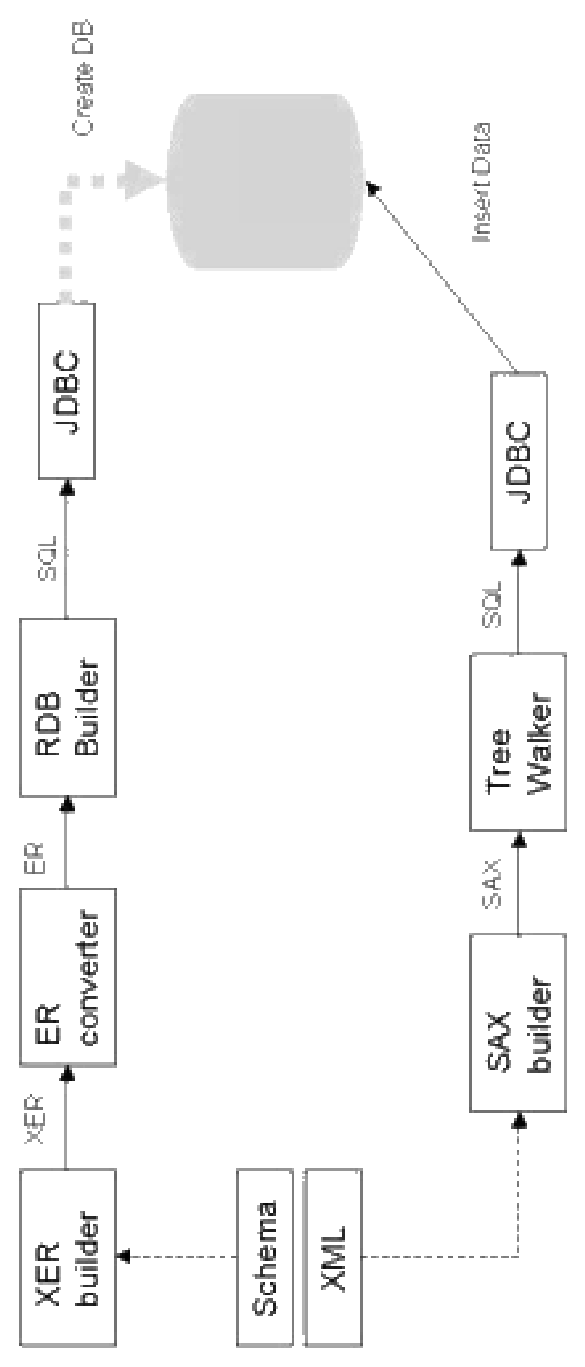
\includegraphics[angle=270,scale=0.5]{control-flow.eps}
\caption{The flow of control during the translation of an XML Document to Relational Data}
\label{control_flow}
\end{center}
\end{figure}

\subsection{Graphical User Interface}

I have briefly considered which GUI toolkit I wish to use to build a user interface, which is likely to take the form of a wizard. With past experience of Swing applications' poor speed, I am keen to use a lighter and faster GUI toolkit. IBM's SWT toolkit seems the likely choice. However, I am also keen to retain cross-plaform compatibility and am currently uncertain of the extent to which SWT supports this.

In addition, I would like the GUI to have at least a simple view of the Relational Database into which data has been imported, and hence I have been looking for a Database Viewer API.

\section{Further Information}

\begin{itemize}
\item This project is being supervised by Peter McBrien. 
\item The project webpage is available at: {\tt http://www.doc.ic.ac.uk/\~&ss401/project/}. I have listed meetings and my latest activities. The report is also avaiable in pdf format.
\end{itemize}

%\begin{thebibliography}{99}
    ....
    \bibitem{DandJ} Dow, W. \& Jones, E.A.,
   {\it Wall Street Journal},
     March 29, 1929.
    ....
    \end{thebibliography}



\end{document}
